\chapter{剩余}

\begin{introduction}
\item 二次互反律
\item 勒让德符号
\item 二次剩余
\item N次剩余
\end{introduction}

\vbox{}

第三章中我们已经知道了如何解线性同余式,现在让我们来考虑更高次的同余方程,首先来看下二次同余方程。

\section{二次剩余}
在发现规律前,人们总要先做一些实验。取模数为7,取遍底数:
$$
\begin{aligned} 0^{2} & \equiv 0(\bmod 7) \\ 1^{2} & \equiv 1(\bmod 7) \\ 2^{2} & \equiv 4(\bmod 7) \\ 3^{2} & \equiv 2(\bmod 7) \\ 4^{2} & \equiv 2(\bmod 7) \\ 5^{2} & \equiv 4(\bmod 7) \\ 6^{2} & \equiv 1(\bmod 7) \end{aligned}
$$

我们可以看到余数并不会包含所有底数,而且不包含的还挺多。

再取多一点模数,如图\ref{fig:quadratic-residue-example}。

\begin{figure}[htbp]
	\centering
	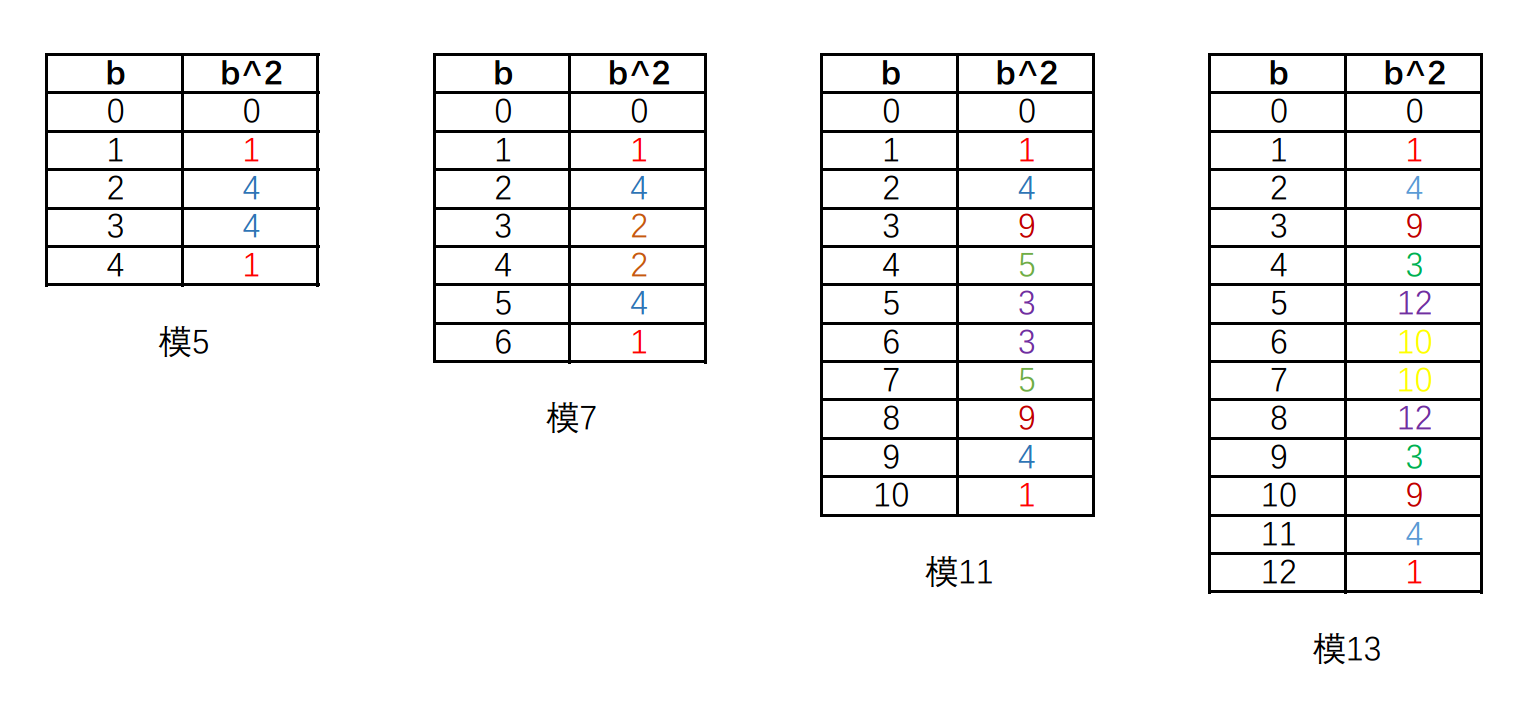
\includegraphics[width=1.0\textwidth]{quadratic-residue-example.png}
	\caption{二次剩余的模式 \label{fig:quadratic-residue-example}}
\end{figure}

可以看到上下的对称性,即数$b$的平方剩余与数$p-b$的平方剩余是模$p$相同的。这一点也比较好证明:
$$
p^2+b^2-2pb=(p-b)^2\equiv b^2 \quad (mod \ p)
$$

因此,若要列出模$p$的所有(非零)平方剩余,只需要计算出其中的一半:

$$
1^2\ (mod \ p)\ ,\ 2^2\ (mod \ p)\ ,\ ...\ ,\ (\frac{p-1}{2})^2 \ (mod \ p)
$$

那如何快速判断一个数是否是二次剩余呢?在探索之前,我们先明确一下定义:

\begin{definition}{二次剩余与二次非剩余}{label}
\begin{itemize}
\item 与一个平方数模$p$同余的非零数称为模$p$的二次剩余
\item 不与任何一个平方数模$p$同余的数称为模$p$的二次非剩余
\item 将二次剩余简记为$QR$,二次非剩余简记为$NR$
\item 与0模$p$同余的数既不是$QR$,也不是$NR$
\end{itemize}
\end{definition}


\begin{theorem}{二次剩余性质}{label}
设$p$为一个奇素数,则恰有$\frac{p-1}{2}$个模$p$的二次剩余,且恰有$\frac{p-1}{2}$个模$p$的二次非剩余。
\end{theorem}

\begin{proof}
由前面的结论知道,只要证明$1^2,2^2,...,(\frac{p-1}{2})^2  \ mod \ p$是两两不同的。

假设$b_1,b_2$是$[1,\frac{p-1}{2}]$之间的数,且满足$b_1^2\equiv b_2^2\ (mod \ p)$。

我们要证明$b_1=b_2$。

由于$b_1^2\equiv b_2^2\ (mod \ p)$,得到$p\ | \ (b_1^2-b_2^2)=(b_1-b_2)(b_1+b_2)$,

然而$b1+b2$显然不能被$p$整除,所以$b_1-b_2=0$,证毕。
\end{proof}

\vbox{}

QR与NR有什么关系呢?一个不难想到的结论是$QR*QR=QR$。(等于号表示仍为$QR$)
因为平方数乘平方数仍为平方数,所以两个二次剩余乘积模$p$仍为二次剩余。那么其他的组合呢?
经过一些小的表观察,可以得到:

$$
QR*QR=QR  ,\quad QR*NR=NR  ,\quad NR*NR=QR
$$

在验证后面两个关系之前,我们先来看下原根与二次剩余的关系,原根是分析一些问题时好用的工具,
也许能帮助我们证明。

设$g$是模$p$的一个原根,那么$g$的幂:
\begin{align}
g\ ,\ g^2\ ,\ g^3\ ,\ ...\ ,\ g^{p-1} \label{formula:primeroot-residue}
\end{align}

可以给出$p$的所有非零剩余,即$[1,p-1]$。其中一半是二次剩余,一半是二次非剩余。
如何确定哪些是$QR$,哪些是$NR$呢?

显然$g$的每个偶次幂一定是一个$QR$,即$g^{2k}$。

注意到在式子\ref{formula:primeroot-residue}中恰有一半是偶次幂,所以{\heiti $g$的偶次幂给出了所有的二次剩余}。而剩下的奇次幂必定是二次非剩余。

同时,也可以用指标来描述,二次剩余是指标$I(a)$为偶数的那些数$a$;二次非剩余是指标$I(a)$为奇数的那些数$a$。
利用二次剩余与二次非剩余的这种指标性质,可以很简单地证明二次剩余的乘法法则。

\begin{theorem}{二次剩余乘法法则--表达方式1}{residue1}
设$p$为素数,则
\begin{itemize}
\item 两个模$p$的二次剩余的积是二次剩余
\item 二次剩余与二次非剩余的积是二次非剩余
\item 两个二次非剩余的积是二次剩余
\end{itemize}
即
$$
QR*QR=QR  ,\quad QR*NR=NR  ,\quad NR*NR=QR
$$
\end{theorem}

\begin{proof}
对与$p\ (p>2)$互素的任意两个数$a,b$,由指标的乘积法则知$I(ab)\equiv I(a)+I(b) \quad (mod \ p-1)$,
从而有$I(ab)\equiv I(a)+I(b) \quad (mod \ 2)$。 后面的证明就很自然了。可以讨论定理\ref{thm:residue1}中的三种情况。
\end{proof}

\vbox{}

对于定理\ref{thm:residue1},你肯定会想到$QR,NR$和$+1,-1$的性质类似。
许多年前,勒让德(Adrien-Marie Legendre)也想到了,而且还引入了一种符号:


\begin{definition}{勒让德符号}{label}
$a$模$p$的勒让德符号是
\begin{align*}
\left(\frac{a}{p}\right)=\left\{\begin{matrix}
1 & \quad  if\ a\ is\ Quadratic\ residue \\  
-1& \quad  else
\end{matrix}\right.
\end{align*}
\end{definition}

利用勒让德符号,二次剩余的乘法法则可用一个公式表示。

\begin{theorem}{二次剩余乘法法则--表达方式2}{residue2}
设$p$为素数,则
$$
\left(\frac{a}{p}\right)\left(\frac{b}{p}\right)=\left(\frac{ab}{p}\right)
$$
\end{theorem}

勒让德符号使计算可以更直观,比如
$$
\left(\frac{75}{97}\right)=\left(\frac{3\cdot5\cdot5}{97}\right)=\left(\frac{3}{97}\right)\left(\frac{5}{97}\right)\left(\frac{5}{97}\right)
$$
而
$$
\left(\frac{5}{97}\right)\left(\frac{5}{97}\right)=1
$$
所以
$$
\left(\frac{75}{97}\right)=\left(\frac{3}{97}\right)=1 \quad   (3\ is\ QR)
$$

这里能够判断出3是模97的一个$QR$有些幸运($10^2$),我们似乎还没有回答如何快速计算一个数是否是二次剩余,即如何快速计算勒让德符号。

\section{二次互反律}
通过前一节的讨论,我们清楚了对于任何一个奇素数,$[1,p-1]$有一半是二次剩余。
现在先换个角度,考虑对于一个数$a$,看看对于哪些$p$,这个数是$QR$。

我们先令$a=-1$,看对于哪些素数$p$,同余式$x^2\equiv -1\ (mod \ p)$有解。
或者说,对哪些素数,$\left( \frac{-1}{p} \right)=1$。同样,通过列出小的数据,可以看出,
{\heiti 若$p$与1模4同余,则$-1$似乎是$p$的$QR$;若$p$与3模4同余,则$-1$似乎是$NR$。}

用来证明这个猜想的工具称为“费马小定理的平方根”,即考虑$A=a^\frac{p-1}{2} \ mod \ p$值为多少?

\begin{theorem}{欧拉准则}{label}
设$p$为素数,则
$$
a^\frac{p-1}{2}\equiv  \left( \frac{a}{p} \right) \quad mod \ p
$$
\end{theorem}

\begin{proof}
令$A=a^\frac{p-1}{2}$,显然$A^2\equiv 1 \ mod \ p$,因此$p$整除$(A-1)(A+1)$。
从而$p$要么整除$(A-1)$要么整除$(A+1)$,因此$A$要么和$1$模$p$同余,要么和$-1$。


当$a$是$QR$时,则$a\equiv g^{2k}\ (mod \ p)$ ,则$a^{\frac{p-1}{2}}\equiv (g^{p-1})^k\equiv 1\ (mod \ p)$;
当$a$是$NR$时,则$a\equiv g^{2k+1} \ (mod \ p)$,则$a^{\frac{p-1}{2}}\equiv g^{\frac{p-1}{2}} \ (mod \ p)$。
由前面讨论知道,$a^{\frac{p-1}{2}}$要么和$1$模$p$同余,要么和$-1$。这里由于$g$是原根,则和$1$模$p$同余的最小次幂只能是$p-1$。
所以这里$a^{\frac{p-1}{2}}\equiv -1 \ (mod \ p)$。
证毕。
\end{proof}


有了欧拉准则,就可以轻松的判断$-1$是不是$p$的二次剩余了:

\begin{theorem}{二次互反律---part one}{label}

设$p$为素数,{\heiti 若$p$与1模4同余,则$-1$是$p$的$QR$;若$p$与3模4同余,则$-1$是$NR$。}

用勒让德符号表示如下:
$$
\left(  \frac{-1}{p}  \right)= \left\{\begin{matrix}
1   \quad if\ p\equiv 1 \ (mod \ 4) \\ 
-1 \quad if\ p\equiv 3 \ (mod \ 4)
\end{matrix}\right.
$$
\end{theorem}

\begin{proof}
带入欧拉准则即证。
\end{proof}

\vbox{}

下面考虑$a=2$的情况。如果直接使用欧拉准则,即$2^{\frac{p-1}{2}} \ mod \ p$,似乎不能看出结果是1还是-1。
高斯提出了一个方法,可以简单地知道$2^{\frac{p-1}{2}} \ mod \ p$的值是-1还是1,其结论和二次互反律part one一样简单:


\begin{theorem}{二次互反律---part two}{label}
$$
\left(  \frac{2}{p}  \right)= \left\{\begin{matrix}
1   \quad if\ p\equiv 1\ or\ 7 \ (mod \ 8) \\ 
-1 \quad if\ p\equiv 3\ or\ 5\ (mod \ 8)
\end{matrix}\right.
$$
\end{theorem}

\begin{proof}
利用欧拉准则知,需要寻找$2^{\frac{p-1}{2}} \ mod \ p$结果的模式。
$p$是一个素数,令$P=\frac{p-1}{2}$,从偶数$2,4,6,...,p-1$开始,将它们相乘,并从每个数中提出2因子,可得
$$
2*4*6*\cdots*(p-1)=2^P*P!
$$
然后再对$2,4,6,...,p-1$进行模$p$化简,使其全部落在$[-P,P]$之间,乘起来。比较这两个乘积,可得
$$
2^P*P!\equiv (-1)^{Number\ of\ negative\ signs}* P! \quad (mod \ p)
$$
负号的个数是指对$2,4,6,...,p-1$进行模$p$化简后落在$[-P,-1]$之间的个数。消去$P!$,得
$$
2^{\frac{p-1}{2}}\equiv  (-1)^{Number\ of\ negative\ signs}  \quad  (mod \ p)
$$
于是当负数的个数为偶数时,$2$是$p$的二次剩余。而这里负数的个数和$p\ mod\ 8$相关,具体如定理中所示。
\end{proof}

\vbox{}

现在总结一下。对于一个给定的数$a$,我们要确定哪些素数$p$以$a$为二次剩余。上面解决了$a=-1$和$a=2$时的问题。
这个时候我们可以通过查看$p\%m$的一些结果得出$a$是否是$QR$或$NR$,且$m$较小,为$4$和$8$。
下面要解决的是其他$a$值的勒让德符号$(\frac{a}{p})$的计算问题。({\heiti 当然,你可以直接使用欧拉准则
去计算},但下面的方法还是很值得知晓)

例如,假设要计算$(\frac{70}{p})$,由前面的二次剩余乘法法则知,$(\frac{70}{p})=(\frac{2}{p})(\frac{5}{p})(\frac{7}{p})$,
怎么计算$(\frac{5}{p})$和$(\frac{7}{p})$呢?

概括来说,怎么计算$(\frac{q}{p})$呢?其中$q$也为素数。因为由乘法法则知,素数可以解决后,整数都可以解决。

通过打表观察后(此处略去500字......),可以得到对于一些$p,q$,有$\left( \frac{q}{p} \right)=\left( \frac{p}{q} \right)$;但有些不是,但不是的竟然都是$\left( \frac{q}{p} \right)=-\left( \frac{p}{q} \right)$。
这其中有没有模式呢?有的。

\begin{theorem}{二次互反律}{label}
$$
\left(  \frac{-1}{p}  \right)= \left\{\begin{matrix}
1   \quad if\ p\equiv 1 \ (mod \ 4) \\ 
-1 \quad if\ p\equiv 3 \ (mod \ 4)
\end{matrix}\right.
$$
$$
\left(  \frac{2}{p}  \right)= \left\{\begin{matrix}
1   \quad if\ p\equiv 1\ or\ 7 \ (mod \ 8) \\ 
-1 \quad if\ p\equiv 3\ or\ 5\ (mod \ 8)
\end{matrix}\right.
$$
$$
\left(\frac{q}{p}\right)=\left\{\begin{array}{c}{\left(\frac{p}{q}\right)}\quad if\ p\equiv1\ (mod\ 4)\ or\ q\equiv1\ (mod\ 4) \\ {-\left(\frac{p}{q}\right) \quad if\ p\equiv3\ (mod\ 4)\ and\ q\equiv3\ (mod\ 4) }\end{array}\right.
$$
\end{theorem}

\begin{proof}
前两部分已经证明,最后一个部分感兴趣的读者可以自行查阅资料。
\end{proof}

\vbox{}

二次互反律不仅很美,也很实用。
它使我们可以翻转勒让德符号$\left(\frac{q}{p}\right)$,用$\pm \left(\frac{p}{q}\right)$来替代它,然后可以模$q$化简$p$,并不断重复此过程,这样会使$p,q$急剧下降。

所以,计算勒让德符号的困难之处不是二次互反律的使用,而是对数字的因式分解。

如果不分解,继续做下去,这样答案是否正确呢?

{\heiti 正确!} 也就是说对于$\left(\frac{q}{p}\right)$,之前是$p,q$为素数,现在是对任意的正奇数$a$和$b$,可以给勒让德符号$\left(\frac{a}{b}\right)$指定一个值,反复使用广义二次互反定律来计算结果。这种广义勒让德符号常称作{\heiti 雅克比符号}。

\begin{theorem}{广义二次互反律}{label}
设$a,b$为正奇数,则
$$
\left(  \frac{-1}{b}  \right)= \left\{\begin{matrix}
1   \quad if\ b\equiv 1 \ (mod \ 4) \\ 
-1 \quad if\ b\equiv 3 \ (mod \ 4)
\end{matrix}\right.
$$
$$
\left(  \frac{2}{b}  \right)= \left\{\begin{matrix}
1   \quad if\ b\equiv 1\ or\ 7 \ (mod \ 8) \\ 
-1 \quad if\ b\equiv 3\ or\ 5\ (mod \ 8)
\end{matrix}\right.
$$
$$
\left(\frac{a}{b}\right)=\left\{\begin{array}{c}{\left(\frac{b}{a}\right)}\quad if\ a\equiv1\ (mod\ 4)\ or\ b\equiv1\ (mod\ 4) \\ {-\left(\frac{b}{a}\right) \quad if\ a\equiv3\ (mod\ 4)\ and\ b\equiv3\ (mod\ 4) }\end{array}\right.
$$
\end{theorem}

\begin{note}
只允许当$a$是正奇数的时候翻转$a,b$,这一点极为重要。当$a$是偶数时,可以分解出因子2;当$a$是负数时,可以分解出因子$-1$。
\end{note}

\vbox{}

使用二次互反律求解勒让德符号,时间复杂度  $O(logb)$。

{\heiti 当然也可以直接用欧拉准则,快速幂即可。}

\lstinputlisting[language=C++, style=codestyle2]{code04/Legendre.cpp}

现在我们可以快速计算勒让德符号了(两种方法)。{\heiti 但知道有解还是不够的,往往我们想知道解是什么。}


\section{求解二次剩余}
Cipolla's algorithm是求解二次剩余的经典方法。
\begin{theorem}{Cipolla's algorithm}{Cipolla}
现有同余式$x^2\equiv n\ (mod\ p)$,其中$x,n\in \mathcal{F}_p$,$p$是奇素数,$\mathcal{F}_p$是有$p$个元素的有限域:$\{0,1,...,p-1\}$。
\begin{enumerate}
\item 寻找一个$a\in \mathcal{F}_p$,使得$a^2-n$是非二次剩余。(随机寻找即可,期望随机次数为2)
\item 在域$\mathcal{F}_{p^2}=\mathcal{F}_p(\sqrt{a^2-n})$中计算$x = (a+\sqrt{a^2-n})^{(p+1)/2}$即为满足$x^2=n$的一个解。
\end{enumerate}
\end{theorem}

在证明前,我们先来看一个例子。注意第二步骤之前所有元素都是在域$\mathcal{F}_{13}$中,第二步中在域$\mathcal{F}_{13^2}$中。

寻找$x^2=10$的所有解。

在执行算法前,你可以先用欧拉准则或者二次互反律计算一下$\left(  \frac{10}{13}  \right)$是否为1,若不是1,则无解;若是1,执行下面算法。

\begin{enumerate}
\item 随机寻找一个$a\in \mathcal{F}_{13}$,使得$a^2-10$是非二次剩余。假如随机到$a=2$,则$a^2-10$为$7$,$\left(  \frac{7}{13}  \right)=-1$,
满足要求。
\item 计算$x = (a+\sqrt{a^2-n})^{(p+1)/2} = (2+\sqrt{-6})^7$。
$$
\begin{array}{l}{(2+\sqrt{-6})^{2}=4+4 \sqrt{-6}-6=-2+4 \sqrt{-6}} \\ {(2+\sqrt{-6})^{4}=(-2+4 \sqrt{-6})^{2}=-1-3 \sqrt{-6}} \\ {(2+\sqrt{-6})^{6}=(-2+4 \sqrt{-6})(-1-3 \sqrt{-6})=9+2 \sqrt{-6}} \\ {(2+\sqrt{-6})^{7}=(9+2 \sqrt{-6})(2+\sqrt{-6})=6}\end{array}
$$
所以$x=6$是一个解,当然$(-6)\ mod\ 13 = 7$也是一个解。
\end{enumerate}

\vbox{}

\begin{proof}
Cipolla's algorithm正确性的证明。

{\heiti Part I\quad 证明$\mathcal{F}_{p^2}=\mathcal{F}_p(\sqrt{a^2-n})=\{x+y\sqrt{a^2-n}:x,y\in \mathcal{F}_p\}$确实是一个域。}

为了记号方便,令$\omega = \sqrt{a^2-n}$,由于$a^2-n$是非二次剩余,所以在$\mathcal{F}_{p}$中是没有平方根的。这里$\omega$可以类比复数域中的$i$。

$\mathcal{F}_{p^2}$中的加法被定义为:
$$
\left(x_{1}+y_{1} \omega\right)+\left(x_{2}+y_{2} \omega\right)=\left(x_{1}+x_{2}\right)+\left(y_{1}+y_{2}\right) \omega
$$

乘法被定义为:
$$
\left(x_{1}+y_{1} \omega\right)\left(x_{2}+y_{2} \omega\right)=x_{1} x_{2}+x_{1} y_{2} \omega+y_{1} x_{2} \omega+y_{1} y_{2} \omega^{2}=\left(x_{1} x_{2}+y_{1} y_{2}\left(a^{2}-n\right)\right)+\left(x_{1} y_{2}+y_{1} x_{2}\right) \omega
$$

可交换、可结合、可分配都比较显然。加法幺元是$0+0\omega$,乘法幺元是$1+0\omega$。
下面证明加法和乘法逆元的存在。显然$x+y\omega$的加法逆元是$-x-y\omega$。对于乘法,记$\alpha = x_1+y_1\omega,\ \alpha^{-1}=x_{2}+y_{2} \omega$,则有:
$$
\left(x_{1}+y_{1} \omega\right)\left(x_{2}+y_{2} \omega\right)=\left(x_{1} x_{2}+y_{1} y_{2}\left(a^{2}-n\right)\right)+\left(x_{1} y_{2}+y_{1} x_{2}\right) \omega=1
$$

通过对应系数可得两个方程:
$$
\left\{\begin{array}{l}{x_{1} x_{2}+y_{1} y_{2}\left(a^{2}-n\right)=1} \\ {x_{1} y_{2}+y_{1} x_{2}=0}\end{array}\right.
$$

解得:
$$
\begin{array}{l}{x_{2}=-y_{1}^{-1} x_{1}\left(y_{1}\left(a^{2}-n\right)-x_{1}^{2} y_{1}^{-1}\right)^{-1}} \\ {y_{2}=\left(y_{1}\left(a^{2}-n\right)-x_{1}^{2} y_{1}^{-1}\right)^{-1}}\end{array}
$$

也就是说$x_2,\ y_2$确实存在,因为其表达式中的元素均在$\mathcal{F}_{p}$中。

Part I证毕,$\mathcal{F}_{p^2}$确实是一个域。

\vbox{}

{\heiti Part II\quad 证明对于域中的每个元素,有$x+y \omega \in \mathcal{F}_{p^{2}}:(x+y \omega)^{p}=x-y \omega$。}

首先在模$p$意义下有$(a+b)^p = a^p + b^p$,$x^p=x$,$\omega^{p-1}=\left(\omega^{2}\right)^{\frac{p-1}{2}}=-1 \ $ ($\omega^2=a^2-n$是非二次剩余,欧拉准则)。
所以
$$
(x+y \omega)^{p}=x^{p}+y^{p} \omega^{p}=x-y \omega
$$

Part II证毕。

\vbox{}

{\heiti Part III\quad 证明若$x_{0}=(a+\omega)^{\frac{p+1}{2}} \in \mathcal{F}_{p^{2}}$,则有$x_{0}^{2}=n \in \mathcal{F}_{p}$。}

$$
x_{0}^{2}=(a+\omega)^{p+1}=(a+\omega)(a+\omega)^{p}=(a+\omega)(a-\omega)=a^{2}-\omega^{2}=a^{2}-\left(a^{2}-n\right)=n
$$

注意上面的计算都发生在域$\mathcal{F}_{p^{2}}$中,所以$x_0\in \mathcal{F}_{p^{2}}$。由拉格朗日定理,在任何域上,$n$阶多项式最多有$n$个根。在$\mathcal{F}_{p}$上,$x^2-n$有两个
根,这些根在$\mathcal{F}_{p^{2}}$上同样也是根。所以在$\mathcal{F}_{p^{2}}$上$x^2-n$的两个根$x_0,\ -x_0$也是$\mathcal{F}_{p}$上$x^2-n$的根。

Part III证毕。

更多资料可以查看\href{https://en.wikipedia.org/wiki/Cipolla\%27s_algorithm}{https://en.wikipedia.org/wiki/Cipolla\%27s\_algorithm}
\end{proof}

\vbox{}

{\heiti 时间复杂度:$O(logp)$,常数较大,因为域$\mathcal{F}_{p^{2}}$中运算取模较多。}

模数为素数。
\lstinputlisting[language=C++, style=codestyle2]{code04/quad-res.cpp}

\vbox{}

{\heiti 如果模数是质数幂呢?}

设$q=p^k$,考虑求解$x^2\equiv n\ (mod\ q)$。当$n\equiv 0\ (mod\ p^k)$时,解为$x \equiv 0\left(\bmod p^{\lceil k / 2\rceil}\right)$。
否则可令$n=p^{r} a,\ p \nmid a,\ 0 \leqslant r<k$,有解时需要$r$为偶数,令$x=p^{r/2}x'$,则$x'^2\equiv a\ (mod\ p^{k-r})$。

所以只要考虑$x^2\equiv a\ (mod\ q)$,且$p\nmid a$的情况即可。下面分$p=2$和$p>2$两种情况讨论。

\begin{enumerate}
\item {\heiti 模2的幂。}$x^{2} \equiv a(\bmod\ q), q=2^{k}, 2\nmid a$。$q=4$时,有解当且仅当$a\equiv 1\ (mod\ 4)$,解为$x\equiv 1,3\ (mod\ 4)$。

下面考虑$q\ge8$的情况。由于任意奇数的平方模$8$余1,于是需有$a\equiv 1\ (mod\ 8)$。此时,$x^2\equiv a\ (mod\ q)$恰有4个解$\pm x_{k}, \pm\left(q / 2-x_{k}\right)$。
\begin{proof}
$q=8$时,4个解分别为$x \equiv \pm 1, \pm 3(\bmod 8)$。下面进行归纳。设$x^{2} \equiv a\left(\bmod\ 2^{k}\right)$的4个解为$\pm x_{k}, \pm\left(2^{k-1}-x_{k}\right)$,则
$$
\begin{aligned} & x_{k}^{2}-\left(2^{k-1}-x_{k}\right)^{2} \\=&\left(2 x_{k}-2^{k-1}\right) 2^{k-1} \\ \equiv & x_{k} 2^{k} \quad\left(\bmod\ 2^{k+1}\right) \\ \equiv & 2^{k} \quad\left(\bmod\ 2^{k+1}\right) \end{aligned}
$$
于是$x_{k}, 2^{k-1}-x_{k}$中恰有一个可以作为$x_{k+1}$,使得$x_{k+1}^{2} \equiv a\left(\bmod\ 2^{k+1}\right)$。又由$\left(2^{k}-x_{k+1}\right)^{2} \equiv x_{k+1}^{2}\left(\bmod\ 2^{k+1}\right)$即得另外两个解。证毕。
\end{proof}

\item {\heiti 模奇素数的幂。}$x^{2} \equiv a(\bmod\ q), q=p^{k}, p \nmid a$。当且仅当$a$是$p$的二次剩余时,上式有解。有解时恰有两个解$\pm x_{k}$。
\begin{proof}
使用归纳法。若$x_{k}^{2} \equiv a\left(\bmod\ p^{k}\right)$,设
$$
\begin{aligned} x_{k+1} &=x_{k}+t p^{k}\left(\bmod\ p^{k+1}\right), t=0,1, \cdots, p-1 \\ x_{k+1}^{2} &=x_{k}^{2}+t^{2} p^{2 k}+2 x_{k} t p^{k} \\ & \equiv x_{k}^{2}+2 x_{k} t p^{k}\left(\bmod\ p^{k+1}\right) \\ & \equiv a\left(\bmod\ p^{k+1}\right) \end{aligned}
$$
于是
$$
2x_kt\equiv (a-x_k^2)/p^k\ (mod\ p)
$$
解出$t$即可得到对应的$x_{k+1}$。
证毕。
\end{proof}
\end{enumerate}

\vbox{}

{\heiti 如果模数是合数,将模数分解后分别计算,再用中国剩余定理合并。}

参考资料:\href{https://max.book118.com/html/2018/0525/168640677.shtm}{jcvb\quad 二次剩余相关}

\section{求解N次剩余}
\begin{custom}{问题}
	给定$N,a,p$,求出$x^N\equiv a\ (mod \ p)$在模$p$意义下的所有解(其中$p$是素数) 。
\end{custom}

\begin{solution}
	如果能找到原根$g$,则$\{1,2,..,.p-1\}$与$\{g^1,g^2,...,g^{p-1}\}$之间就建立了双射关系。
	
	令$g^y=x,\ g^t=a$,$x^N\equiv a\ (mod \ p)$ ,则有
	$$
	g^{y*N}\equiv g^t  \quad (mod \ p)
	$$
	因为$p$是素数,所以方程左右都不会为0。原问题转化为:
	$$
	N*y\equiv t\ (mod \ (p-1))
	$$
	由于$N,p$已知,则上式为解模线性方程。
	
	而$t$的值,由$g^t\equiv a \ (mod\ p)$,用解离散对数的方法求出。
\end{solution}

输入:$1 \le a,\ N < p \le 10^9$,$p$为素数。

{\heiti 时间复杂度}  $O(\sqrt{p}log(\sqrt{p}))$ 

\lstinputlisting[language=C++, style=codestyle2]{code04/N-res.cpp}

{\heiti 如果模数是非素数呢?}

模数非素数:时间和素数一样,甚至更低,因为分解质因数处理的时候规模较小,最后中国剩余定理合并。
\lstinputlisting[language=C++, style=codestyle2]{code04/N-res-notprime.cpp}

\begin{example}
	已知$x^{2^{30}+3}\ mod\ n = c$,给定$c,n$,其中$n$是两个相邻素数($p \in [10^5, 10^9]$)的乘积。求解$x$,题目保证在模意义下只有一个解。
	$10^5$组测试数据。
	(\href{https://codeforces.com/gym/102055/problem/K}{CCPC2018-Final Mr. Panda and Kakin})
\end{example}

\begin{solution}
	注意到这里$2^{30}+3$和$\phi(n)$一定互质,所以可以直接求$2^{30}+3$模$\phi(n)$下的逆元,最后两边做逆元次方即得答案。
	
	注意要使用$O(1)$快速乘,否则超时。
\end{solution}

\lstinputlisting[language=C++, style=codestyle2]{code04/Kakin.cpp}


\vbox{}

\vbox{}

\begin{problemset}
	\item \href{https://www.luogu.org/problem/P5491}{二次剩余 \quad 洛谷P5491 \quad 模板}
	\item \href{https://www.51nod.com/Challenge/Problem.html#problemId=1123}{任意模数N次剩余 \quad 51nod 1123 \quad 模板}
\end{problemset}